%% 
%% Copyright 2019-2021 Elsevier Ltd
%% 
%% This file is part of the 'CAS Bundle'.
%% --------------------------------------
%% 
%% It may be distributed under the conditions of the LaTeX Project Public
%% License, either version 1.2 of this license or (at your option) any
%% later version.  The latest version of this license is in
%%    http://www.latex-project.org/lppl.txt
%% and version 1.2 or later is part of all distributions of LaTeX
%% version 1999/12/01 or later.
%% 
%% The list of all files belonging to the 'CAS Bundle' is
%% given in the file `manifest.txt'.
%% 
%% Template article for cas-dc documentclass for 
%% double column output.

\documentclass[fleqn]{cas-sc}

\usepackage{lipsum}
\usepackage{tikz}
\usetikzlibrary{shapes, snakes, calc}

% If the frontmatter runs over more than one page
% use the longmktitle option.

%\documentclass[a4paper,fleqn,longmktitle]{cas-dc}

%\usepackage[numbers]{natbib}
%\usepackage[authoryear]{natbib}
\usepackage[authoryear,longnamesfirst]{natbib}

%%%Author macros
\def\tsc#1{\csdef{#1}{\textsc{\lowercase{#1}}\xspace}}
\tsc{WGM}
\tsc{QE}
%%%

% Uncomment and use as if needed
%\newtheorem{theorem}{Theorem}
%\newtheorem{lemma}[theorem]{Lemma}
%\newdefinition{rmk}{Remark}
%\newproof{pf}{Proof}
%\newproof{pot}{Proof of Theorem \ref{thm}}

\begin{document}
\let\WriteBookmarks\relax
\def\floatpagepagefraction{1}
\def\textpagefraction{.001}

% Short title
\shorttitle{Ambulance Dispatch}    

% Short author
\shortauthors{Burkman, Jin, and Sun}  

% Main title of the paper
\title [mode = title]{Modeling the Need for an Ambulance based on Automated Crash Reports from iPhones}  

% Title footnote mark
% eg: \tnotemark[1]
%\tnotemark[<tnote number>] 
%\tnotemark[1] 

% Title footnote 1.
% eg: \tnotetext[1]{Title footnote text}
%\tnotetext[1]{Working Title} 

% First author
%
% Options: Use if required
% eg: \author[1,3]{Author Name}[type=editor,
%       style=chinese,
%       auid=000,
%       bioid=1,
%       prefix=Sir,
%       orcid=0000-0000-0000-0000,
%       facebook=<facebook id>,
%       twitter=<twitter id>,
%       linkedin=<linkedin id>,
%       gplus=<gplus id>]

%\author[<aff no>]{<author name>}[<options>]
\author[1,2]{J. Bradford Burkman}[]
% Footnote of the first author
%\fnmark[1]
% Corresponding author indication
\cormark[1]
% Email id of the first author
\ead{bradburkman@gmail.com}
% URL of the first author
\ead[url]{www.lsmsa.edu}

% Credit authorship
% eg: \credit{Conceptualization of this study, Methodology, Software}
% Options: conceptualization; data curation; formal analysis; funding acquisition; investigation; methodology; project administration; resources; software; supervision; validation; visualization; writing – original draft; and writing – review and editing.
\credit{Conceptualization, Investigation, Writing - original draft, Visualization}


\author[1]{Miao Jin}[]
\credit{Supervision, Methodology, Writing - review and editing}

\author[3]{Xiaoduan Sun}[]
\credit{Data curation, Writing - review and editing}






\affiliation[1]{organization={School of Computing and Informatics, University of Louisiana at Lafayette},
%            addressline={301 E. Lewis St}, 
%            city={Lafayette},
%          citysep={}, % Uncomment if no comma needed between city and postcode
%            state={LA},
%            postcode={70503}, 
            country={USA}}

% Address/affiliation
\affiliation[2]{organization={Louisiana School for Math, Science, and the Arts},
%            addressline={715 University Pkwy}, 
%            city={Natchitoches},
%          citysep={}, % Uncomment if no comma needed between city and postcode
%            state={LA},
%            postcode={71457}, 
            country={USA}}

\affiliation[3]{organization={Department of Civil Engineering, University of Louisiana at Lafayette},
%            addressline={131 Rex St}, 
%            city={Lafayette},
%          citysep={}, % Uncomment if no comma needed between city and postcode
%            state={LA},
%            postcode={70504}, 
            country={USA}}




% For a title note without a number/mark
%\nonumnote{}

% Here goes the abstract
\begin{abstract}
%%%%% Abstract
% I found an abstract in TRpC June 2022 with 365 words.
Put abstract here.
\vskip 1in

\end{abstract}

% Use if graphical abstract is present
%\begin{graphicalabstract}
%\includegraphics{}
%\end{graphicalabstract}

% Research highlights
\begin{highlights}
	\item  Supports transferability and benchmarking of different approaches on a public large-scale dataset.  The associated GitHub page provides the code and detailed notes used to perform the analysis on the Crash Report Sampling System.  
	\item Novel Application:  Machine Learning Classification Models for Dispatching Ambulances based on Automated Crash Reports
	\item Perennial Machine Learning Challenge:  Imbalanced Datasets, more challenging because we use two similar datasets with different imbalances.
	\item 
\end{highlights}

% Keywords
% Each keyword is seperated by \sep
\begin{keywords}
 \sep Automated crash notification \sep Ambulance dispatch \sep Emergency medical services  \sep Machine learning
\end{keywords}

\maketitle

% Main text

%%%%% Introduction
\section{Introduction}\label{What does the label do?}

\begin{comment}
	Notes from 5/16/22 meeting with Dr. Jin:
		I Motivation - Good, needs more material
		II Analyze Difficulty in Solving Problem
		III ML/Data Analysis
			Tradeoffs
			Limits of Methods
		IV Plan
		
		Mention overlaps with other work
\end{comment}

%%%
\subsection{Motivation}


%Starting in 2022, each new iPhone has a feature that can automatically notify police if the phone detects the deceleration profile of a crash.  If the injuries are serious, time to medical care is critical, but few crashes result in serious injuries, and ambulances are in limited supply and expensive.  From the data available from such an automatic notification, can we build a machine-learning model that will recommend whether police should immediately, perhaps automatically, dispatch an ambulance?  

A Google Pixel phone can detect the deceleration profile of a car crash and, if you have enabled the settings in the Personal Safety app, will, if you do not respond in 60 seconds, automatically call the police, reporting your location.  Apple announced in November 2021 that it was planning to do something similar.  

The crash victims who would most obviously benefit from such technology are those in crashes with no witnesses to call police (``unnoticed run-off roadway''), who survived the crash, and might have lived if help had arrived promptly, but died from their injuries.  Such crashes, though, are very rare, about seventy-seven fatalities annually in the US in 2010-2018,   
\citep{SPICER2021105974}
of the about 35,000 crash fatalities per year in the same time period.  \citep{FARS}
% 2020:  38,824
% 2019:  36,355
% 2018:  36,835
% 2017:  37,473
% 2016:  37,806
% 2015:  35,484
% 2014:  32,744
% 2013:  32,893
% 2012:  33,782
% 2011:  32,479
% 2010:  32,999

A much larger group who could benefit from  are those injuries are serious and need prompt medical attention.  Dispatching an ambulance automatically, rather than waiting for an eyewitness to call for one, would cut at least several minutes off of the ambulance response time.  In a 1996 study on 1990 data for US urban interstates, freeways, and expressways \citep{edsoai.on1047979037n.d.}, the average accident notification time was 5.2 minutes, and the additional time to EMS (emergency medical services) arrival was 6.2 minutes.    Evanco estimated that reducing the notification time from 5.2 minutes to 2 minutes would cut fatalities by 15.9\%.   Even those who might not die may recover more fully and quickly with prompt medical attention, so dispatching an ambulance promptly when one is needed would be beneficial.  

On the other hand, we do not want to send an ambulance to every accident scene, because only a small proportion of crashes have severe injury; most are property damage only (PDO) crashes.  Ambulances and their crews are expensive and in finite supply.  

Given the information available to the police from a phone's automated crash notification, can we build a model that will recommend (or determine) whether to send an ambulance immediately?  





\input{Intro_Datasets}
%%%
\subsection{Difficulty in Solving Problem}

Such a model will not be perfect, with some false negatives (not sending an ambulance when one is needed) and many false positives (sending an ambulance when one is not needed).  We will show that the quality of the model depends largely on what information is available.  Some information (location, time of day, day of week, weather) either comes with the automated report or is easy to get.  Other information (age and sex of phone's primary user, vehicle likely to be driven by that person) may be very helpful in predicting injury, but getting that information would require instantaneous communication between private and public databases.  Being able to interpret the location, ({\it e.g.} Is that precise location inside an intersection of two roads with high speed limits?) in real time would require planning and preparation.  

The problem is both political and ethical as well as technical.  How many false positives will we tolerate to have one fewer false negative?  We will show that, given such a marginal tolerance $p$, we can incorporate that tradeoff into the model, but each locality will have to decide that for itself.  Implementing such a system would require budgets, cooperation, and possibly legislation, but knowing which data is most useful can help set priorities.  



%%%
\subsection{Machine Learning Challenges}

We deal with several machine learning challenges in our study, and their solutions are often as much art as science.  

\begin{description}

	\item [Feature Selection]  We need to select the features most relevant to crash severity; too many less-relevant features will muddle the model building.  CRSS has both ``Make'' and ``Body Type.''  Do these two features give enough different information 
that we should use both?  If not, which is more useful?

\item [Feature Engineering]
We can also merge features into useful new features.  In both data sets, we have ``Day of Week'' and ``Hour.''  We would like to take from each to make ``Rush Hour,'' if it has a different hospitalization profile.  When does it start and end?  Is morning rush hour different from evening?  Does it start earlier on Fridays?  

\item [Binning]
Some features have many values that we can usefully combine into bins or bands.  The \verb|AGE| feature has values 0-120.   A simple approach would be to put it in decade bands, but in most states in the US, the driving age is 16.  The crash severity profiles for new drivers are different than for experienced drivers, so a split at 15/16 makes sense.  In our analysis, the crash severity profiles for ages 52-70 are similar to each other but different from 71+, so we broke them into bands there.  
	
\item [Missing Data]  As with all real data, many samples (records) have missing values.  The CRSS authors imputed missing values in some but not all features, for historical reasons going back to 1982.  \citep{CRSS_Imputation}  We compared their method with two others and imputed missing values in all of the features we used.  

\item [Imbalanced Data]	
Only a small proportion of crashes require immediate medical attention.  In the CRSS data, about 15\% of persons involved in a crash were transported by ambulance.  If we built a model that classified all crashes as ``Ambulance Not Needed,'' the model would have 85\% accuracy, which would be excellent in some other applications, but not here.  The toolkit for building models on imbalanced data is well established, but many of the tools only work for continuous data (our data is all categorical).
	
	
\end{description}



%%%
\subsection{Research Plan}

\begin{enumerate}
	\item On both raw data sets, do cleanup, feature selection, and feature engineering.  To the extent possible, make the two engineered data sets the same.
	\item Starting with the easiest-to-obtain data (general location, time/day, weather), and interatively adding more data (persons, vehicles, specific location), build and evaluate a model that predicts whether an ambulance is needed.
	\item Combine results from the two datasets.
	\item Interpret and discuss how the model improves as more data becomes available.  
\end{enumerate}

%%%%% Lit Review
\section{Literature Review}
\input{Lit_Review}

%%%%% Methods
%%%%%
%\section{Methods}

%We have written this section as a guide for other to replicate and adapt our work, so some details may seem pedantic.

\subsection{Metrics}\label{Methods_Metrics}

{\bf Precision} tells us, of the ambulances we sent, how many were needed.  {\bf Recall} tells us, of the ambulances that were needed, how many we sent.  Recall only looks at elements of the minority class (positive class, ``need ambulance''), so is independent of the class imbalance.  Precision is affected by class imbalance, but is still relevant to our decisions in its imbalanced form.  Because the number of elements of the positive class in the test set is constant across all of our models, recall is proportional to TP. 

The {\bf F1 score} is the harmonic mean of precision and recall. Why the harmonic mean instead of the arithmetic or geometric?  For two positive numbers $a$ and $b$ with $0 < a < b$, 
$$a < Harm(a,b) < Geo(a,b) < Arith(a,b) < b$$
so the F1 score emphasizes what the model does poorly.  We will use F1 as our primary indicator, while looking at precision and recall.  

The area under the curve ({\bf AUC}) of the receiver operating characteristic (ROC) is a measure of how well a model separates the samples of the positive and negative classes.  We will use it to show that the additional features in the ``hard/expensive'' and ``medium'' datasets are important for discriminating between the two classes.  

The $\Delta FP/\Delta TP$ curve is related to the ROC; $\Delta FP/\Delta TP$ is the reciprocal of the product of the slope of the ROC curve and a factor that corrects for class imbalance. 

%$$mROC = \frac{\Delta TPR}{\Delta FPR} = \frac{\frac{\Delta TP}{P}}{\frac{\Delta FP}{N}} = \frac{N}{P} \cdot \frac{\Delta TP}{\Delta FP} = \frac{1}{ \frac{P}{N} \cdot \frac{\Delta FP}{\Delta TP}}$$

$$
\frac{\Delta FP}{\Delta TP} = 
\frac{N}{P} \cdot \frac{\frac{\Delta FP}{N}}{\frac{\Delta TP}{P}}
= \frac{N}{P} \cdot \frac{\Delta FPR}{\Delta TPR}
= \frac{1}{\frac{P}{N} \cdot \frac{\Delta TPR}{\Delta FPR}}
= \frac{1}{\frac{P}{N} \cdot mROC}
$$
 We will use this curve to find the value of the discrimination threshold where $\Delta FP/\Delta TP = 2.0$



%%%
\subsection{ Incorporating the $\Delta FP/\Delta TP < \omega$ Ethical Threshold}

We incorporated this ethical threshold in two ways, as a class weight and as the decision threshold.  

\subsubsection{Class Weight}

To understand why class weights can encode this threshold, we will use the $\alpha$-weighted binary crossentropy model as an example.  

To move the model towards $\Delta FP/\Delta TP < \omega \to \Delta FP - \omega\Delta TP < 0$ is equivalent to minimizing $FP - \omega TP$.  The $\alpha$-weighted binary crossentropy loss function is 

$$\displaystyle Loss = - \left(\alpha \sum_{y=1} \log \left( h_\theta (x_i) \right) + (1-\alpha) \sum_{y=0} \log \left(1 - h_\theta(x_i)\right)  \right)$$

In this function, $y_i \in \{0,1\}$ is the ground truth for sample $i$, 0 if in the majority class (''no ambulance'') and 1 if in the minority class (``yes ambulance'').  The term $h_\theta(x_i)\in [0,1]$ is the probability that $x_i$ is in the minority class, as calculated by this $\theta$ iteration of the model.

The TN, FP, FN, and TP are discrete, and the $h_\theta(x_i)$ is continuous.  To see how they relate, let us discretize the loss function, with 

$$
\log\left(h_\theta(x_i)\right) \to 
\begin{cases}
	0 & \text{if } h_\theta(x_i) \le 0.5 \cr
	1 & \text{if } h_\theta(x_i) > 0.5 \cr
\end{cases}
\text{\quad and \quad}
\log\left(1 - h_\theta(x_i)\right) \to 
\begin{cases}
	0 & \text{if } 1 - h_\theta(x_i) \le 0.5 \cr
	1 & \text{if } 1 - h_\theta(x_i) > 0.5 \cr
\end{cases}
$$

\noindent which makes $\displaystyle \sum_{y=1} \log ( h_\theta (x_i) )$ into $TP$ and  $\displaystyle \sum_{y=0} \log(1 - h_\theta(x_i))$ into $TN$, making the discrete version of the loss function
$$Loss = -\left(\alpha TP + (1-\alpha) TN\right)$$

In the following manipulations, note that adding a constant, or multiplying by a positive constant, does not change the effect of the loss function, which the model algorithm uses to compare one iteration to the next.

\

\hfil \begin{tabular}{ >{$\displaystyle}r<{$} @{\hspace{3pt}}>{$\displaystyle}c<{$} @{\hspace{3pt}}>{$\displaystyle}l<{$} l <{\vrule width 0pt height 12pt depth 12pt} }
	Loss &=& -\left(\alpha TP + (1-\alpha) TN\right) &\cr
	Loss &=& -\left(\frac{\omega}{\omega +1} TP + \frac{1}{\omega +1} TN\right) &Let $\displaystyle\alpha = \frac{\omega}{\omega +1}$, making $\displaystyle1 - \alpha = \frac{1}{\omega +1}$ \cr
	Loss &=& -\left( \omega \cdot TP + TN \right) & Multiply by $\omega+1$ \cr
	Loss &=& -\left( \omega \cdot TP + TN \right) + TN + FP & Add constant $TN+FP$, the number of majority samples\cr
	Loss &=& FP - \omega \cdot TP & \cr
\end{tabular}

Thus, we can incorporate the ethical threshold $p$ into our loss function as the class weight.  For this study we have arbitrarily chosen $\omega = 2$, so we will use class weight $\alpha = \omega/(\omega+1) = 2/3$.

%%%
\subsubsection{Decision Threshold}

Once a supervised learning algorithm learns a model using the training set, it evaluates the model on the test set, returning for each sample in the test set a probability $p\in [0,1]$ that the sample belongs to the positive class (``need ambulance'').  By default we use a decision threshold $p=0.5$ to discriminate between predicted negative (PN) and predicted positive (PP), but for good cause we can choose a different threshold.  We will choose to make the decision threshold the value of $p$ that makes $\Delta FP/\Delta TP = 2$.  Because many tools are built around having the decision threshold at $p=0.5$, rather than change the decision threshold we will linearly transform the probabilities $p \in [0,1]$ to shift the desired threshold of $p$ where $\Delta FP/\Delta TP = 2$ to $p=0.5$.  

Consider these results from one of our models.  The histogram shows, for the negative (``no ambulance'') and positive (``ambulance'') classes, the percentage of the dataset in each range of $p$.  In an ideal model, the negative class would be clustered on the left and the positive on the right.  The ROC curve and the area under the curve (AUC) indicates how cleanly the model separates the two classes, with $AUC=1$ being perfect and $AUC=0.5$ being basically random classification.


\

%%%
\parbox{\linewidth}{
%{\bf Balanced Random Forest model, Hard features, No Tomek, $\alpha = 2/3$}

\noindent\hspace{-6pt}\input{../Keras/Images/Ideal_Shift_to_FP_equals_r_TP_Pred_Wide.pgf}
	
\noindent\begin{tabular}{@{\hspace{-6pt}}p{2.3in} @{\hspace{-6pt}}p{2.0in} p{1.8in}}
	\vskip 0pt
	\hfil Raw Model Output
	
%	\input{../Keras/Images/KBFC_Hard_Tomek_2_alpha_target_gamma_0_0_v2_Pred.pgf}	
&
	\vskip 0pt
	\hfil ROC Curve
	
%	\input{../Keras/Images/KBFC_Hard_Tomek_2_alpha_target_gamma_0_0_v2_ROC.pgf}
	
&
	\vskip 0pt
	\begin{tabular}{cc|c|c|}
	&\multicolumn{1}{c}{}& \multicolumn{2}{c}{Prediction} \cr
	&\multicolumn{1}{c}{} & \multicolumn{1}{c}{N} & \multicolumn{1}{c}{P} \cr\cline{3-4}
	\multirow{2}{*}{\rotatebox[origin=c]{90}{Actual}}&N &
118,776 & 31,995
	\vrule width 0pt height 10pt depth 2pt \cr\cline{3-4}
	&P & 
10,572 & 16,049
	\vrule width 0pt height 10pt depth 2pt \cr\cline{3-4}
	\end{tabular}

	\hfil\begin{tabular}{ll}
	\cr
0.334 & Precision \cr	0.603 & Recall \cr	0.430 & F1 \cr
\end{tabular}

\cr
\end{tabular}
} % End parbox

\

Mapping $\Delta FP/\Delta TP$ as a function of $p$ for this model, we see that it equals $\omega = 2$ when $p = 0.720$.  Using a linear transformation, we can map $0.720$ to $0.5$, keeping 0 at 0, to get transformed model output with the decision threshold where $\Delta FP/\Delta TP = 2$.  The ROC curve and its AUC are invariant under such a transformation.  

\

%%%
\parbox{\linewidth}{
%{\bf Balanced Random Forest model, Hard features, No Tomek, $\alpha = 2/3$}

\noindent\begin{tabular}{@{\hspace{-6pt}}p{2.3in} @{\hspace{-6pt}}p{2.0in} p{1.8in}}
	\vskip 0pt
	\qquad $\Delta FP/\Delta TP$ as a function of $p$
	
%	%% Creator: Matplotlib, PGF backend
%%
%% To include the figure in your LaTeX document, write
%%   \input{<filename>.pgf}
%%
%% Make sure the required packages are loaded in your preamble
%%   \usepackage{pgf}
%%
%% Also ensure that all the required font packages are loaded; for instance,
%% the lmodern package is sometimes necessary when using math font.
%%   \usepackage{lmodern}
%%
%% Figures using additional raster images can only be included by \input if
%% they are in the same directory as the main LaTeX file. For loading figures
%% from other directories you can use the `import` package
%%   \usepackage{import}
%%
%% and then include the figures with
%%   \import{<path to file>}{<filename>.pgf}
%%
%% Matplotlib used the following preamble
%%   
%%   \usepackage{fontspec}
%%   \makeatletter\@ifpackageloaded{underscore}{}{\usepackage[strings]{underscore}}\makeatother
%%
\begingroup%
\makeatletter%
\begin{pgfpicture}%
\pgfpathrectangle{\pgfpointorigin}{\pgfqpoint{2.247807in}{1.754444in}}%
\pgfusepath{use as bounding box, clip}%
\begin{pgfscope}%
\pgfsetbuttcap%
\pgfsetmiterjoin%
\definecolor{currentfill}{rgb}{1.000000,1.000000,1.000000}%
\pgfsetfillcolor{currentfill}%
\pgfsetlinewidth{0.000000pt}%
\definecolor{currentstroke}{rgb}{1.000000,1.000000,1.000000}%
\pgfsetstrokecolor{currentstroke}%
\pgfsetdash{}{0pt}%
\pgfpathmoveto{\pgfqpoint{0.000000in}{0.000000in}}%
\pgfpathlineto{\pgfqpoint{2.247807in}{0.000000in}}%
\pgfpathlineto{\pgfqpoint{2.247807in}{1.754444in}}%
\pgfpathlineto{\pgfqpoint{0.000000in}{1.754444in}}%
\pgfpathlineto{\pgfqpoint{0.000000in}{0.000000in}}%
\pgfpathclose%
\pgfusepath{fill}%
\end{pgfscope}%
\begin{pgfscope}%
\pgfsetbuttcap%
\pgfsetmiterjoin%
\definecolor{currentfill}{rgb}{1.000000,1.000000,1.000000}%
\pgfsetfillcolor{currentfill}%
\pgfsetlinewidth{0.000000pt}%
\definecolor{currentstroke}{rgb}{0.000000,0.000000,0.000000}%
\pgfsetstrokecolor{currentstroke}%
\pgfsetstrokeopacity{0.000000}%
\pgfsetdash{}{0pt}%
\pgfpathmoveto{\pgfqpoint{0.530556in}{0.499444in}}%
\pgfpathlineto{\pgfqpoint{2.080556in}{0.499444in}}%
\pgfpathlineto{\pgfqpoint{2.080556in}{1.654444in}}%
\pgfpathlineto{\pgfqpoint{0.530556in}{1.654444in}}%
\pgfpathlineto{\pgfqpoint{0.530556in}{0.499444in}}%
\pgfpathclose%
\pgfusepath{fill}%
\end{pgfscope}%
\begin{pgfscope}%
\pgfsetbuttcap%
\pgfsetroundjoin%
\definecolor{currentfill}{rgb}{0.000000,0.000000,0.000000}%
\pgfsetfillcolor{currentfill}%
\pgfsetlinewidth{0.803000pt}%
\definecolor{currentstroke}{rgb}{0.000000,0.000000,0.000000}%
\pgfsetstrokecolor{currentstroke}%
\pgfsetdash{}{0pt}%
\pgfsys@defobject{currentmarker}{\pgfqpoint{0.000000in}{-0.048611in}}{\pgfqpoint{0.000000in}{0.000000in}}{%
\pgfpathmoveto{\pgfqpoint{0.000000in}{0.000000in}}%
\pgfpathlineto{\pgfqpoint{0.000000in}{-0.048611in}}%
\pgfusepath{stroke,fill}%
}%
\begin{pgfscope}%
\pgfsys@transformshift{0.601010in}{0.499444in}%
\pgfsys@useobject{currentmarker}{}%
\end{pgfscope}%
\end{pgfscope}%
\begin{pgfscope}%
\definecolor{textcolor}{rgb}{0.000000,0.000000,0.000000}%
\pgfsetstrokecolor{textcolor}%
\pgfsetfillcolor{textcolor}%
\pgftext[x=0.601010in,y=0.402222in,,top]{\color{textcolor}\rmfamily\fontsize{10.000000}{12.000000}\selectfont 0.008}%
\end{pgfscope}%
\begin{pgfscope}%
\pgfsetbuttcap%
\pgfsetroundjoin%
\definecolor{currentfill}{rgb}{0.000000,0.000000,0.000000}%
\pgfsetfillcolor{currentfill}%
\pgfsetlinewidth{0.803000pt}%
\definecolor{currentstroke}{rgb}{0.000000,0.000000,0.000000}%
\pgfsetstrokecolor{currentstroke}%
\pgfsetdash{}{0pt}%
\pgfsys@defobject{currentmarker}{\pgfqpoint{0.000000in}{-0.048611in}}{\pgfqpoint{0.000000in}{0.000000in}}{%
\pgfpathmoveto{\pgfqpoint{0.000000in}{0.000000in}}%
\pgfpathlineto{\pgfqpoint{0.000000in}{-0.048611in}}%
\pgfusepath{stroke,fill}%
}%
\begin{pgfscope}%
\pgfsys@transformshift{2.024334in}{0.499444in}%
\pgfsys@useobject{currentmarker}{}%
\end{pgfscope}%
\end{pgfscope}%
\begin{pgfscope}%
\definecolor{textcolor}{rgb}{0.000000,0.000000,0.000000}%
\pgfsetstrokecolor{textcolor}%
\pgfsetfillcolor{textcolor}%
\pgftext[x=2.024334in,y=0.402222in,,top]{\color{textcolor}\rmfamily\fontsize{10.000000}{12.000000}\selectfont 0.97}%
\end{pgfscope}%
\begin{pgfscope}%
\definecolor{textcolor}{rgb}{0.000000,0.000000,0.000000}%
\pgfsetstrokecolor{textcolor}%
\pgfsetfillcolor{textcolor}%
\pgftext[x=1.305556in,y=0.223333in,,top]{\color{textcolor}\rmfamily\fontsize{10.000000}{12.000000}\selectfont \(\displaystyle p\)}%
\end{pgfscope}%
\begin{pgfscope}%
\pgfsetbuttcap%
\pgfsetroundjoin%
\definecolor{currentfill}{rgb}{0.000000,0.000000,0.000000}%
\pgfsetfillcolor{currentfill}%
\pgfsetlinewidth{0.803000pt}%
\definecolor{currentstroke}{rgb}{0.000000,0.000000,0.000000}%
\pgfsetstrokecolor{currentstroke}%
\pgfsetdash{}{0pt}%
\pgfsys@defobject{currentmarker}{\pgfqpoint{-0.048611in}{0.000000in}}{\pgfqpoint{-0.000000in}{0.000000in}}{%
\pgfpathmoveto{\pgfqpoint{-0.000000in}{0.000000in}}%
\pgfpathlineto{\pgfqpoint{-0.048611in}{0.000000in}}%
\pgfusepath{stroke,fill}%
}%
\begin{pgfscope}%
\pgfsys@transformshift{0.530556in}{0.540910in}%
\pgfsys@useobject{currentmarker}{}%
\end{pgfscope}%
\end{pgfscope}%
\begin{pgfscope}%
\definecolor{textcolor}{rgb}{0.000000,0.000000,0.000000}%
\pgfsetstrokecolor{textcolor}%
\pgfsetfillcolor{textcolor}%
\pgftext[x=0.363889in, y=0.492715in, left, base]{\color{textcolor}\rmfamily\fontsize{10.000000}{12.000000}\selectfont \(\displaystyle {0}\)}%
\end{pgfscope}%
\begin{pgfscope}%
\pgfsetbuttcap%
\pgfsetroundjoin%
\definecolor{currentfill}{rgb}{0.000000,0.000000,0.000000}%
\pgfsetfillcolor{currentfill}%
\pgfsetlinewidth{0.803000pt}%
\definecolor{currentstroke}{rgb}{0.000000,0.000000,0.000000}%
\pgfsetstrokecolor{currentstroke}%
\pgfsetdash{}{0pt}%
\pgfsys@defobject{currentmarker}{\pgfqpoint{-0.048611in}{0.000000in}}{\pgfqpoint{-0.000000in}{0.000000in}}{%
\pgfpathmoveto{\pgfqpoint{-0.000000in}{0.000000in}}%
\pgfpathlineto{\pgfqpoint{-0.048611in}{0.000000in}}%
\pgfusepath{stroke,fill}%
}%
\begin{pgfscope}%
\pgfsys@transformshift{0.530556in}{0.946322in}%
\pgfsys@useobject{currentmarker}{}%
\end{pgfscope}%
\end{pgfscope}%
\begin{pgfscope}%
\definecolor{textcolor}{rgb}{0.000000,0.000000,0.000000}%
\pgfsetstrokecolor{textcolor}%
\pgfsetfillcolor{textcolor}%
\pgftext[x=0.294444in, y=0.898128in, left, base]{\color{textcolor}\rmfamily\fontsize{10.000000}{12.000000}\selectfont \(\displaystyle {20}\)}%
\end{pgfscope}%
\begin{pgfscope}%
\pgfsetbuttcap%
\pgfsetroundjoin%
\definecolor{currentfill}{rgb}{0.000000,0.000000,0.000000}%
\pgfsetfillcolor{currentfill}%
\pgfsetlinewidth{0.803000pt}%
\definecolor{currentstroke}{rgb}{0.000000,0.000000,0.000000}%
\pgfsetstrokecolor{currentstroke}%
\pgfsetdash{}{0pt}%
\pgfsys@defobject{currentmarker}{\pgfqpoint{-0.048611in}{0.000000in}}{\pgfqpoint{-0.000000in}{0.000000in}}{%
\pgfpathmoveto{\pgfqpoint{-0.000000in}{0.000000in}}%
\pgfpathlineto{\pgfqpoint{-0.048611in}{0.000000in}}%
\pgfusepath{stroke,fill}%
}%
\begin{pgfscope}%
\pgfsys@transformshift{0.530556in}{1.351735in}%
\pgfsys@useobject{currentmarker}{}%
\end{pgfscope}%
\end{pgfscope}%
\begin{pgfscope}%
\definecolor{textcolor}{rgb}{0.000000,0.000000,0.000000}%
\pgfsetstrokecolor{textcolor}%
\pgfsetfillcolor{textcolor}%
\pgftext[x=0.294444in, y=1.303540in, left, base]{\color{textcolor}\rmfamily\fontsize{10.000000}{12.000000}\selectfont \(\displaystyle {40}\)}%
\end{pgfscope}%
\begin{pgfscope}%
\definecolor{textcolor}{rgb}{0.000000,0.000000,0.000000}%
\pgfsetstrokecolor{textcolor}%
\pgfsetfillcolor{textcolor}%
\pgftext[x=0.238889in,y=1.076944in,,bottom,rotate=90.000000]{\color{textcolor}\rmfamily\fontsize{10.000000}{12.000000}\selectfont \(\displaystyle \Delta\)FP/\(\displaystyle \Delta\)TP}%
\end{pgfscope}%
\begin{pgfscope}%
\pgfpathrectangle{\pgfqpoint{0.530556in}{0.499444in}}{\pgfqpoint{1.550000in}{1.155000in}}%
\pgfusepath{clip}%
\pgfsetrectcap%
\pgfsetroundjoin%
\pgfsetlinewidth{1.505625pt}%
\definecolor{currentstroke}{rgb}{0.000000,0.000000,0.000000}%
\pgfsetstrokecolor{currentstroke}%
\pgfsetdash{}{0pt}%
\pgfpathmoveto{\pgfqpoint{0.601010in}{1.601944in}}%
\pgfpathlineto{\pgfqpoint{0.615243in}{1.561939in}}%
\pgfpathlineto{\pgfqpoint{0.629477in}{1.519987in}}%
\pgfpathlineto{\pgfqpoint{0.643710in}{1.480900in}}%
\pgfpathlineto{\pgfqpoint{0.657943in}{1.443667in}}%
\pgfpathlineto{\pgfqpoint{0.672176in}{1.408434in}}%
\pgfpathlineto{\pgfqpoint{0.686410in}{1.330371in}}%
\pgfpathlineto{\pgfqpoint{0.700643in}{1.267651in}}%
\pgfpathlineto{\pgfqpoint{0.714876in}{1.207433in}}%
\pgfpathlineto{\pgfqpoint{0.729109in}{1.151946in}}%
\pgfpathlineto{\pgfqpoint{0.743343in}{1.099513in}}%
\pgfpathlineto{\pgfqpoint{0.757576in}{1.052935in}}%
\pgfpathlineto{\pgfqpoint{0.771809in}{1.014007in}}%
\pgfpathlineto{\pgfqpoint{0.786042in}{0.979069in}}%
\pgfpathlineto{\pgfqpoint{0.800276in}{0.948758in}}%
\pgfpathlineto{\pgfqpoint{0.814509in}{0.922183in}}%
\pgfpathlineto{\pgfqpoint{0.828742in}{0.898615in}}%
\pgfpathlineto{\pgfqpoint{0.842975in}{0.877569in}}%
\pgfpathlineto{\pgfqpoint{0.857209in}{0.857331in}}%
\pgfpathlineto{\pgfqpoint{0.871442in}{0.838338in}}%
\pgfpathlineto{\pgfqpoint{0.885675in}{0.822090in}}%
\pgfpathlineto{\pgfqpoint{0.899908in}{0.807805in}}%
\pgfpathlineto{\pgfqpoint{0.914142in}{0.794292in}}%
\pgfpathlineto{\pgfqpoint{0.928375in}{0.781980in}}%
\pgfpathlineto{\pgfqpoint{0.942608in}{0.770643in}}%
\pgfpathlineto{\pgfqpoint{0.956841in}{0.760249in}}%
\pgfpathlineto{\pgfqpoint{0.971075in}{0.750603in}}%
\pgfpathlineto{\pgfqpoint{0.985308in}{0.741532in}}%
\pgfpathlineto{\pgfqpoint{0.999541in}{0.734003in}}%
\pgfpathlineto{\pgfqpoint{1.013774in}{0.727075in}}%
\pgfpathlineto{\pgfqpoint{1.028007in}{0.720197in}}%
\pgfpathlineto{\pgfqpoint{1.042241in}{0.713595in}}%
\pgfpathlineto{\pgfqpoint{1.056474in}{0.707399in}}%
\pgfpathlineto{\pgfqpoint{1.070707in}{0.701829in}}%
\pgfpathlineto{\pgfqpoint{1.084940in}{0.696135in}}%
\pgfpathlineto{\pgfqpoint{1.099174in}{0.690924in}}%
\pgfpathlineto{\pgfqpoint{1.113407in}{0.685834in}}%
\pgfpathlineto{\pgfqpoint{1.127640in}{0.681070in}}%
\pgfpathlineto{\pgfqpoint{1.141873in}{0.676223in}}%
\pgfpathlineto{\pgfqpoint{1.156107in}{0.671763in}}%
\pgfpathlineto{\pgfqpoint{1.170340in}{0.667671in}}%
\pgfpathlineto{\pgfqpoint{1.184573in}{0.663708in}}%
\pgfpathlineto{\pgfqpoint{1.198806in}{0.659965in}}%
\pgfpathlineto{\pgfqpoint{1.213040in}{0.656061in}}%
\pgfpathlineto{\pgfqpoint{1.227273in}{0.652540in}}%
\pgfpathlineto{\pgfqpoint{1.241506in}{0.648888in}}%
\pgfpathlineto{\pgfqpoint{1.255739in}{0.645356in}}%
\pgfpathlineto{\pgfqpoint{1.269973in}{0.641959in}}%
\pgfpathlineto{\pgfqpoint{1.284206in}{0.638769in}}%
\pgfpathlineto{\pgfqpoint{1.298439in}{0.635617in}}%
\pgfpathlineto{\pgfqpoint{1.312672in}{0.632377in}}%
\pgfpathlineto{\pgfqpoint{1.326906in}{0.629137in}}%
\pgfpathlineto{\pgfqpoint{1.341139in}{0.625924in}}%
\pgfpathlineto{\pgfqpoint{1.355372in}{0.623014in}}%
\pgfpathlineto{\pgfqpoint{1.369605in}{0.620208in}}%
\pgfpathlineto{\pgfqpoint{1.383839in}{0.617626in}}%
\pgfpathlineto{\pgfqpoint{1.398072in}{0.615168in}}%
\pgfpathlineto{\pgfqpoint{1.412305in}{0.612747in}}%
\pgfpathlineto{\pgfqpoint{1.426538in}{0.610317in}}%
\pgfpathlineto{\pgfqpoint{1.440771in}{0.607976in}}%
\pgfpathlineto{\pgfqpoint{1.455005in}{0.605820in}}%
\pgfpathlineto{\pgfqpoint{1.469238in}{0.603844in}}%
\pgfpathlineto{\pgfqpoint{1.483471in}{0.602020in}}%
\pgfpathlineto{\pgfqpoint{1.497704in}{0.600118in}}%
\pgfpathlineto{\pgfqpoint{1.511938in}{0.598171in}}%
\pgfpathlineto{\pgfqpoint{1.526171in}{0.596238in}}%
\pgfpathlineto{\pgfqpoint{1.540404in}{0.594428in}}%
\pgfpathlineto{\pgfqpoint{1.554637in}{0.592637in}}%
\pgfpathlineto{\pgfqpoint{1.568871in}{0.590944in}}%
\pgfpathlineto{\pgfqpoint{1.583104in}{0.589243in}}%
\pgfpathlineto{\pgfqpoint{1.597337in}{0.587562in}}%
\pgfpathlineto{\pgfqpoint{1.611570in}{0.585881in}}%
\pgfpathlineto{\pgfqpoint{1.625804in}{0.584099in}}%
\pgfpathlineto{\pgfqpoint{1.640037in}{0.582384in}}%
\pgfpathlineto{\pgfqpoint{1.654270in}{0.580793in}}%
\pgfpathlineto{\pgfqpoint{1.668503in}{0.579207in}}%
\pgfpathlineto{\pgfqpoint{1.682737in}{0.577577in}}%
\pgfpathlineto{\pgfqpoint{1.696970in}{0.575975in}}%
\pgfpathlineto{\pgfqpoint{1.711203in}{0.574368in}}%
\pgfpathlineto{\pgfqpoint{1.725436in}{0.572829in}}%
\pgfpathlineto{\pgfqpoint{1.739670in}{0.571283in}}%
\pgfpathlineto{\pgfqpoint{1.753903in}{0.569752in}}%
\pgfpathlineto{\pgfqpoint{1.768136in}{0.568383in}}%
\pgfpathlineto{\pgfqpoint{1.782369in}{0.567039in}}%
\pgfpathlineto{\pgfqpoint{1.796603in}{0.565658in}}%
\pgfpathlineto{\pgfqpoint{1.810836in}{0.564371in}}%
\pgfpathlineto{\pgfqpoint{1.825069in}{0.563124in}}%
\pgfpathlineto{\pgfqpoint{1.839302in}{0.561940in}}%
\pgfpathlineto{\pgfqpoint{1.853535in}{0.560794in}}%
\pgfpathlineto{\pgfqpoint{1.867769in}{0.559649in}}%
\pgfpathlineto{\pgfqpoint{1.882002in}{0.558559in}}%
\pgfpathlineto{\pgfqpoint{1.896235in}{0.557501in}}%
\pgfpathlineto{\pgfqpoint{1.910468in}{0.556449in}}%
\pgfpathlineto{\pgfqpoint{1.924702in}{0.555475in}}%
\pgfpathlineto{\pgfqpoint{1.938935in}{0.554594in}}%
\pgfpathlineto{\pgfqpoint{1.953168in}{0.553719in}}%
\pgfpathlineto{\pgfqpoint{1.967401in}{0.553250in}}%
\pgfpathlineto{\pgfqpoint{1.981635in}{0.552777in}}%
\pgfpathlineto{\pgfqpoint{1.995868in}{0.552333in}}%
\pgfpathlineto{\pgfqpoint{2.010101in}{0.551944in}}%
\pgfusepath{stroke}%
\end{pgfscope}%
\begin{pgfscope}%
\pgfpathrectangle{\pgfqpoint{0.530556in}{0.499444in}}{\pgfqpoint{1.550000in}{1.155000in}}%
\pgfusepath{clip}%
\pgfsetbuttcap%
\pgfsetroundjoin%
\pgfsetlinewidth{1.505625pt}%
\definecolor{currentstroke}{rgb}{0.000000,0.000000,0.000000}%
\pgfsetstrokecolor{currentstroke}%
\pgfsetdash{{5.550000pt}{2.400000pt}}{0.000000pt}%
\pgfpathmoveto{\pgfqpoint{0.530556in}{0.581451in}}%
\pgfpathlineto{\pgfqpoint{2.080556in}{0.581451in}}%
\pgfusepath{stroke}%
\end{pgfscope}%
\begin{pgfscope}%
\pgfpathrectangle{\pgfqpoint{0.530556in}{0.499444in}}{\pgfqpoint{1.550000in}{1.155000in}}%
\pgfusepath{clip}%
\pgfsetrectcap%
\pgfsetroundjoin%
\pgfsetlinewidth{1.505625pt}%
\definecolor{currentstroke}{rgb}{0.121569,0.466667,0.705882}%
\pgfsetstrokecolor{currentstroke}%
\pgfsetdash{}{0pt}%
\pgfpathmoveto{\pgfqpoint{1.654270in}{0.581451in}}%
\pgfusepath{stroke}%
\end{pgfscope}%
\begin{pgfscope}%
\pgfpathrectangle{\pgfqpoint{0.530556in}{0.499444in}}{\pgfqpoint{1.550000in}{1.155000in}}%
\pgfusepath{clip}%
\pgfsetbuttcap%
\pgfsetroundjoin%
\definecolor{currentfill}{rgb}{0.000000,0.000000,0.000000}%
\pgfsetfillcolor{currentfill}%
\pgfsetlinewidth{1.003750pt}%
\definecolor{currentstroke}{rgb}{0.000000,0.000000,0.000000}%
\pgfsetstrokecolor{currentstroke}%
\pgfsetdash{}{0pt}%
\pgfsys@defobject{currentmarker}{\pgfqpoint{-0.041667in}{-0.041667in}}{\pgfqpoint{0.041667in}{0.041667in}}{%
\pgfpathmoveto{\pgfqpoint{0.000000in}{-0.041667in}}%
\pgfpathcurveto{\pgfqpoint{0.011050in}{-0.041667in}}{\pgfqpoint{0.021649in}{-0.037276in}}{\pgfqpoint{0.029463in}{-0.029463in}}%
\pgfpathcurveto{\pgfqpoint{0.037276in}{-0.021649in}}{\pgfqpoint{0.041667in}{-0.011050in}}{\pgfqpoint{0.041667in}{0.000000in}}%
\pgfpathcurveto{\pgfqpoint{0.041667in}{0.011050in}}{\pgfqpoint{0.037276in}{0.021649in}}{\pgfqpoint{0.029463in}{0.029463in}}%
\pgfpathcurveto{\pgfqpoint{0.021649in}{0.037276in}}{\pgfqpoint{0.011050in}{0.041667in}}{\pgfqpoint{0.000000in}{0.041667in}}%
\pgfpathcurveto{\pgfqpoint{-0.011050in}{0.041667in}}{\pgfqpoint{-0.021649in}{0.037276in}}{\pgfqpoint{-0.029463in}{0.029463in}}%
\pgfpathcurveto{\pgfqpoint{-0.037276in}{0.021649in}}{\pgfqpoint{-0.041667in}{0.011050in}}{\pgfqpoint{-0.041667in}{0.000000in}}%
\pgfpathcurveto{\pgfqpoint{-0.041667in}{-0.011050in}}{\pgfqpoint{-0.037276in}{-0.021649in}}{\pgfqpoint{-0.029463in}{-0.029463in}}%
\pgfpathcurveto{\pgfqpoint{-0.021649in}{-0.037276in}}{\pgfqpoint{-0.011050in}{-0.041667in}}{\pgfqpoint{0.000000in}{-0.041667in}}%
\pgfpathlineto{\pgfqpoint{0.000000in}{-0.041667in}}%
\pgfpathclose%
\pgfusepath{stroke,fill}%
}%
\begin{pgfscope}%
\pgfsys@transformshift{1.654270in}{0.581451in}%
\pgfsys@useobject{currentmarker}{}%
\end{pgfscope}%
\end{pgfscope}%
\begin{pgfscope}%
\pgfsetrectcap%
\pgfsetmiterjoin%
\pgfsetlinewidth{0.803000pt}%
\definecolor{currentstroke}{rgb}{0.000000,0.000000,0.000000}%
\pgfsetstrokecolor{currentstroke}%
\pgfsetdash{}{0pt}%
\pgfpathmoveto{\pgfqpoint{0.530556in}{0.499444in}}%
\pgfpathlineto{\pgfqpoint{0.530556in}{1.654444in}}%
\pgfusepath{stroke}%
\end{pgfscope}%
\begin{pgfscope}%
\pgfsetrectcap%
\pgfsetmiterjoin%
\pgfsetlinewidth{0.803000pt}%
\definecolor{currentstroke}{rgb}{0.000000,0.000000,0.000000}%
\pgfsetstrokecolor{currentstroke}%
\pgfsetdash{}{0pt}%
\pgfpathmoveto{\pgfqpoint{2.080556in}{0.499444in}}%
\pgfpathlineto{\pgfqpoint{2.080556in}{1.654444in}}%
\pgfusepath{stroke}%
\end{pgfscope}%
\begin{pgfscope}%
\pgfsetrectcap%
\pgfsetmiterjoin%
\pgfsetlinewidth{0.803000pt}%
\definecolor{currentstroke}{rgb}{0.000000,0.000000,0.000000}%
\pgfsetstrokecolor{currentstroke}%
\pgfsetdash{}{0pt}%
\pgfpathmoveto{\pgfqpoint{0.530556in}{0.499444in}}%
\pgfpathlineto{\pgfqpoint{2.080556in}{0.499444in}}%
\pgfusepath{stroke}%
\end{pgfscope}%
\begin{pgfscope}%
\pgfsetrectcap%
\pgfsetmiterjoin%
\pgfsetlinewidth{0.803000pt}%
\definecolor{currentstroke}{rgb}{0.000000,0.000000,0.000000}%
\pgfsetstrokecolor{currentstroke}%
\pgfsetdash{}{0pt}%
\pgfpathmoveto{\pgfqpoint{0.530556in}{1.654444in}}%
\pgfpathlineto{\pgfqpoint{2.080556in}{1.654444in}}%
\pgfusepath{stroke}%
\end{pgfscope}%
\begin{pgfscope}%
\pgfsetbuttcap%
\pgfsetmiterjoin%
\definecolor{currentfill}{rgb}{1.000000,1.000000,1.000000}%
\pgfsetfillcolor{currentfill}%
\pgfsetfillopacity{0.800000}%
\pgfsetlinewidth{1.003750pt}%
\definecolor{currentstroke}{rgb}{0.800000,0.800000,0.800000}%
\pgfsetstrokecolor{currentstroke}%
\pgfsetstrokeopacity{0.800000}%
\pgfsetdash{}{0pt}%
\pgfpathmoveto{\pgfqpoint{0.811987in}{1.126667in}}%
\pgfpathlineto{\pgfqpoint{1.983333in}{1.126667in}}%
\pgfpathquadraticcurveto{\pgfqpoint{2.011111in}{1.126667in}}{\pgfqpoint{2.011111in}{1.154444in}}%
\pgfpathlineto{\pgfqpoint{2.011111in}{1.557222in}}%
\pgfpathquadraticcurveto{\pgfqpoint{2.011111in}{1.585000in}}{\pgfqpoint{1.983333in}{1.585000in}}%
\pgfpathlineto{\pgfqpoint{0.811987in}{1.585000in}}%
\pgfpathquadraticcurveto{\pgfqpoint{0.784210in}{1.585000in}}{\pgfqpoint{0.784210in}{1.557222in}}%
\pgfpathlineto{\pgfqpoint{0.784210in}{1.154444in}}%
\pgfpathquadraticcurveto{\pgfqpoint{0.784210in}{1.126667in}}{\pgfqpoint{0.811987in}{1.126667in}}%
\pgfpathlineto{\pgfqpoint{0.811987in}{1.126667in}}%
\pgfpathclose%
\pgfusepath{stroke,fill}%
\end{pgfscope}%
\begin{pgfscope}%
\pgfsetrectcap%
\pgfsetroundjoin%
\pgfsetlinewidth{1.505625pt}%
\definecolor{currentstroke}{rgb}{0.000000,0.000000,0.000000}%
\pgfsetstrokecolor{currentstroke}%
\pgfsetdash{}{0pt}%
\pgfpathmoveto{\pgfqpoint{0.839765in}{1.473889in}}%
\pgfpathlineto{\pgfqpoint{0.978654in}{1.473889in}}%
\pgfpathlineto{\pgfqpoint{1.117543in}{1.473889in}}%
\pgfusepath{stroke}%
\end{pgfscope}%
\begin{pgfscope}%
\definecolor{textcolor}{rgb}{0.000000,0.000000,0.000000}%
\pgfsetstrokecolor{textcolor}%
\pgfsetfillcolor{textcolor}%
\pgftext[x=1.228654in,y=1.425277in,left,base]{\color{textcolor}\rmfamily\fontsize{10.000000}{12.000000}\selectfont \(\displaystyle \Delta FP/\Delta TP\)}%
\end{pgfscope}%
\begin{pgfscope}%
\pgfsetrectcap%
\pgfsetroundjoin%
\pgfsetlinewidth{1.505625pt}%
\definecolor{currentstroke}{rgb}{0.121569,0.466667,0.705882}%
\pgfsetstrokecolor{currentstroke}%
\pgfsetdash{}{0pt}%
\pgfpathmoveto{\pgfqpoint{0.839765in}{1.265555in}}%
\pgfpathlineto{\pgfqpoint{0.978654in}{1.265555in}}%
\pgfpathlineto{\pgfqpoint{1.117543in}{1.265555in}}%
\pgfusepath{stroke}%
\end{pgfscope}%
\begin{pgfscope}%
\pgfsetbuttcap%
\pgfsetroundjoin%
\definecolor{currentfill}{rgb}{0.000000,0.000000,0.000000}%
\pgfsetfillcolor{currentfill}%
\pgfsetlinewidth{1.003750pt}%
\definecolor{currentstroke}{rgb}{0.000000,0.000000,0.000000}%
\pgfsetstrokecolor{currentstroke}%
\pgfsetdash{}{0pt}%
\pgfsys@defobject{currentmarker}{\pgfqpoint{-0.041667in}{-0.041667in}}{\pgfqpoint{0.041667in}{0.041667in}}{%
\pgfpathmoveto{\pgfqpoint{0.000000in}{-0.041667in}}%
\pgfpathcurveto{\pgfqpoint{0.011050in}{-0.041667in}}{\pgfqpoint{0.021649in}{-0.037276in}}{\pgfqpoint{0.029463in}{-0.029463in}}%
\pgfpathcurveto{\pgfqpoint{0.037276in}{-0.021649in}}{\pgfqpoint{0.041667in}{-0.011050in}}{\pgfqpoint{0.041667in}{0.000000in}}%
\pgfpathcurveto{\pgfqpoint{0.041667in}{0.011050in}}{\pgfqpoint{0.037276in}{0.021649in}}{\pgfqpoint{0.029463in}{0.029463in}}%
\pgfpathcurveto{\pgfqpoint{0.021649in}{0.037276in}}{\pgfqpoint{0.011050in}{0.041667in}}{\pgfqpoint{0.000000in}{0.041667in}}%
\pgfpathcurveto{\pgfqpoint{-0.011050in}{0.041667in}}{\pgfqpoint{-0.021649in}{0.037276in}}{\pgfqpoint{-0.029463in}{0.029463in}}%
\pgfpathcurveto{\pgfqpoint{-0.037276in}{0.021649in}}{\pgfqpoint{-0.041667in}{0.011050in}}{\pgfqpoint{-0.041667in}{0.000000in}}%
\pgfpathcurveto{\pgfqpoint{-0.041667in}{-0.011050in}}{\pgfqpoint{-0.037276in}{-0.021649in}}{\pgfqpoint{-0.029463in}{-0.029463in}}%
\pgfpathcurveto{\pgfqpoint{-0.021649in}{-0.037276in}}{\pgfqpoint{-0.011050in}{-0.041667in}}{\pgfqpoint{0.000000in}{-0.041667in}}%
\pgfpathlineto{\pgfqpoint{0.000000in}{-0.041667in}}%
\pgfpathclose%
\pgfusepath{stroke,fill}%
}%
\begin{pgfscope}%
\pgfsys@transformshift{0.978654in}{1.265555in}%
\pgfsys@useobject{currentmarker}{}%
\end{pgfscope}%
\end{pgfscope}%
\begin{pgfscope}%
\definecolor{textcolor}{rgb}{0.000000,0.000000,0.000000}%
\pgfsetstrokecolor{textcolor}%
\pgfsetfillcolor{textcolor}%
\pgftext[x=1.228654in,y=1.216944in,left,base]{\color{textcolor}\rmfamily\fontsize{10.000000}{12.000000}\selectfont (0.720,2)}%
\end{pgfscope}%
\end{pgfpicture}%
\makeatother%
\endgroup%
	
&
	\vskip 0pt
	\hfill Transformed Model Output
	
%	\input{../Keras/Images/KBFC_Hard_Tomek_2_alpha_target_gamma_0_0_v2_Linear_Transform_Pred.pgf}
	
&
	\vskip 0pt
	\begin{tabular}{cc|c|c|}
	&\multicolumn{1}{c}{}& \multicolumn{2}{c}{Prediction} \cr
	&\multicolumn{1}{c}{} & \multicolumn{1}{c}{N} & \multicolumn{1}{c}{P} \cr\cline{3-4}
	\multirow{2}{*}{\rotatebox[origin=c]{90}{Actual}}&N &
142,035 & 8,736
	\vrule width 0pt height 10pt depth 2pt \cr\cline{3-4}
	&P & 
18,549 & 8,072
	\vrule width 0pt height 10pt depth 2pt \cr\cline{3-4}
	\end{tabular}

	\hfil\begin{tabular}{ll}
	\cr
0.480 & Precision \cr	0.303 & Recall \cr	0.372 & F1 \cr	0.774 & AUC \cr
\end{tabular}

\cr
\end{tabular}
} % End parbox

\

It is reasonably to ask, ``How is the transformed model ethically better?  We are only sending 8,072 needed ambulances instead of 16,049.  In the original model, $FP/TP = 31,995/16,049 = 1.994 < 2.0 = \omega$.  How is it better to send half as many needed ambulances?''  Because our ethical tradeoff was not for total number of FP and TP, but for marginal FP and TP.   Going from the original to the transformed model, we have $\Delta FP/\Delta TP = (31,995 - 8,736)/(16,049 - 8,072) = 23,259/7,977 = 2.91$, which is higher than our choice of ethical tradeoff $\omega = 2.0$.  For this model, it is at $p = 0.720$ that we reach our tradeoff point.  

We will use the model outputs transformed to have decision threshold at $\Delta FP/\Delta TP = 2.0$ to compare different models. 

%%%
\subsection{Preparing the Data}

The CRSS data is available \href{https://www.nhtsa.gov/crash-data-systems/crash-report-sampling-system}{online at this link}.  The three main files for each year are {\tt Accident}, {\tt Vehicle}, and {\tt Person}, and one uses the {\tt CASENUM} and \verb|VEH_NO| fields to merge them into one dataset.  

%Next we dropped fields that were just random noise, like \verb|MINUTE| and vehicle identification numbers (VIN), fields that had been collected in only some years, and fields that could not be known at the time of the crash, like the results of a driver drug test.  

\subsubsection{Order of Operations}

To prepare the data we needed to do two things, to bin (discretize) some features and to impute missing data.  We did not know which to do first, so we tested both ways using IVEware \citep{IVEware} for the imputation. The imputation is a stochastic process, and the difference between binning first and imputing first was as small as the difference between running twice with different random seeds.  Since IVEware can only handle up to about forty categories in each categorical field, we had had to bin some fields first either way, so we decided on binning first.  

\subsubsection{Binning}
To bin a field's many categories into fewer categories, sometimes the meaning of the categories was a sufficient guide.  In the \verb|HOSPITAL| field, which we used as our target variable, we were only interested in two values, whether or not the person went to the hospital.  The CRSS field has six values indicating how the person went to the hospital (ground ambulance, air ambulance, ...), and we merged those into one.  For fields where the binning was not so obvious, we looked at how each value in the field correlates to hospitalization.  We wanted to put \verb|AGE| into bands, and looked to divide  where the hospitalization rate changed.  Interestingly, ages 16, 17, and 18 have lower hospitalization rates than ages below or above, so we put them into their own band.  Around age 52 the hospitalization rate started to go up, so we split there.  We binned other fields in a similar way.  

The merging, dropping, and binning are all in the \verb|CRSS_04_Discretize| code.

\subsubsection{Imputing Missing Values}

About 47\% of the samples had unknown values in the thirty-eight fields we use for our analysis.   The CRSS authors imputed unknown values in ten of those fields, another seventeen had no unknown values, but eleven fields we want to use had missing values that were not imputed by CRSS.   The CRSS authors have a very helpful report on their imputation methods.  \citep{CRSS_Imputation}  The reasons why some fields get imputed include historical consistency going back to 1982.  

(See \verb|CRSS_04_5_Count_Missing_Values|)  

When the CRSS authors imputed unknown values for a field, they published two fields, one with the imputed values and one with the values signifying ``Unknown.''  We discarded the imputed fields and compared three methods for imputing missing values.  Impute to Mode assigns to all missing values in a feature the most common value in that feature.  IVEware: Imputation and Variance Estimation Software employs multivariate sequential regression, and is the method the CRSS authors used.  Round Robin Random Forest, like in MissForest, was consistently the most accurate.  We tested the methods by dropping all samples with missing values, randomly deleting (but keeping a copy of) fifteen percent of the known values, imputing, and comparing to the ground truth.  

(See \verb|CRSS_05_Impute_Random_Forest| for details.)

We did not address the question of incorrect data.  

%%%
\subsection{Selecting Features}

We selected three groups of features to see whether more information would improve the model.  

The first group of features held information that the police would already know before receiving a crash notification, like time of day, day of week, and urban/rural.  A crash on a Saturday night in a rural area is far more likely to need an ambulance than one in a city at rush hour, so if no information specific to the crash is available, how well can we predict whether an ambulance is needed?  We thought of this set of features as ``easy'' or ``baseline.''

The second group of features also included specific location and the age and sex of the primary user of the phone.  Is the vehicle in an intersection or in a parking lot?  Did the car end up off the roadway?  What is the speed limit on that road?  Getting that information from the latitude and longitude in the automated report would require instantaneous correlation with detailed maps.  Whether such information significantly improves the model will inform whether policymakers should invest the time and effort to have that information available.  We thought of this information as ``medium'' in cost.

The ``hard'' or ``expensive'' features would require regularly updated maps (work zones, lighting conditions), correlating records to guess which car the cell phone user is driving, and correlating multiple cell phone reports to count how many people are involved.  

We dropped all crashes with a pedestrian, because unlike a tree or other vehicle, hitting a pedestrian may not cause the sudden deceleration that a cell phone could distinguish from sudden braking, so the cell phone likely would not register it as a crash.  

(See \verb|CRSS_06_Build_Model| for details.)


%%%
\subsection{Handling Imbalanced Data}

In our dataset only about fifteen percent of the people needed an ambulance.   If a recommendation system never sent an ambulance, the model would have 85\% accuracy, but be useless.  Most algorithms for training models are designed for balanced data, with half of the samples in each of the negative and positive classes.  With an imbalanced data set we can address the imbalance in four levels:  Resampling the dataset, modifying the loss function, choosing metrics other than accuracy, and using learning methods that account for the imbalance.  

\subsubsection{Resampling the Dataset}

We can balance the dataset by undersampling the majority class (negative, ``No ambulance'') or oversampling the minority class (positive, ``Send Ambulance'').  To balance by undersampling would mean throwing out eighty percent of the majority class, losing valuable information.  A very popular method for oversampling is SMOTE (Synthetic Minority Oversampling TEchnique), which creates new minority samples between existing minority samples, but the ``between'' requires continuous data, and all of our data is discrete or categorical.  What is between a Buick and a Volvo?

Tomek Links is one of the few resampling methods that works for categorical data.  It is a selective undersampling method that removes majority samples that seem out of place.  A Tomek Link is a majority/minority pair that are each others' nearest neighbors, which was the case with about four percent of the majority samples.  We used the Tomek algorithm to remove the majority sample of each Tomek link, undersampling the majority class, and then running it again to remove more that had not been Tomek links in the first undersampling run.   


Consider this two-dimensional training dataset.  The six blue circles represent samples (elements) of the majority negative class (``no ambulance''), and the three red squares represent the minority positive class (``ambulance'').  Samples \#7 and \#1 are each others' nearest neighbors of different classes, so they are Tomek Links and the algorithm deletes \#1.  In a second Tomek run, once \#1 is gone, \#7 and \#2 are Tomek Links, so the method deletes \#2.  


\begin{center}
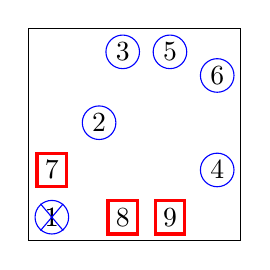
\begin{tikzpicture}[x = 3mm, y=3mm]
	\draw (-1,-1) rectangle (8,8);
	\tikzstyle{Square} = [
		draw = red, 
		very thick,
		rectangle,
		inner sep = 1mm,
		minimum size = 3 mm
	]
	\tikzstyle{SquareFill} = [
		draw = red, 
		fill = red,
		very thick,
		rectangle,
	]
	\tikzstyle{Circle} = [
		draw = blue, 
		circle,
		inner sep = 0.5 mm
	]
	\tikzstyle{CircleFill} = [
		draw = blue,
		fill = blue, 
		circle,
	]
	\node [Circle] (1) at (0,0) {1};
	\node [Circle] (2) at (2,4) {2};
	\node [Circle] (3) at (3,7) {3};
	\node [Circle] (4) at (7,2) {4};
	\node [Circle] (5) at (5,7) {5};
	\node [Circle] (6) at (7,6) {6};
	\node [Square] (7) at (0,2) {7};
	\node [Square] (8) at (3,0) {8};
	\node [Square] (9) at (5,0) {9};

	\node [Circle, cross out] (1) at (0,0) {1};
\end{tikzpicture}
\end{center}



Our original dataset has 619,027 samples.  We first removed the 27,723 crashes involving a pedestrian, leaving 591,304 samples.  Each sample had 82 features; we cut the number of features to 38 for our ``Hard'' features, then to 21 for ``Medium,'' and to 10 for ``Easy.''  We then split each of those three datasets 70/30 into a training set of 413,913 samples and a test set of 177,393 samples, preserving the proportions of negative and positive samples in both sets.  We did the train/test split twice with different random seeds (``Round 1'' and ``Round 2'') to gauge how much of the small differences in results were due to stochasticity instead of differences in the model algorithms or hyperparameters.  Tomek undersampling only applies to the training set, not to the test set.  

We then ran Imbalanced-Learn's  TomekLinks algorithm, then ran it again on the results to give our ``Tomek Once'' and ``Tomek Twice'' undersampled datasets.  

\

\hfil\begin{tabular}{lrrl}
\multicolumn{2}{l}{Hard Features, Round 1}   &  & \cr
 & Samples & \multicolumn{2}{c}{Change} \cr\hline
Original & 413,913 &  & \cr
Tomek Once & 399,515 & 14,398 & 3.48\%\cr
Tomek Twice & 396,511 & 3,004 & 0.75\%\cr\cline{3-4}
Total Change &  & 17,402 & 4.23\%\cr
\end{tabular}
\qquad\begin{tabular}{lrrl}
\multicolumn{2}{l}{Hard Features, Round 2} & \cr
 & Samples & \multicolumn{2}{c}{Change} \cr\hline
Original & 413,913 &  & \cr
Tomek Once & 399,714 & 14,199 & 3.43\%\cr
Tomek Twice & 396,718 & 2,996 & 0.75\%\cr\cline{3-4}
Total Change &  & 17,195 & 4.18\%\cr
\end{tabular}

\vskip 12pt

\hfil\begin{tabular}{lrrl}
\multicolumn{3}{l}{Medium Features, Round 1} & \cr
 & Samples & \multicolumn{2}{c}{Change} \cr\hline
Original & 413,913 &  & \cr
Tomek Once & 406,691 & 7,222 & 1.74\%\cr
Tomek Twice & 405,288 & 1,403 & 0.34\%\cr\cline{3-4}
Total Change &  & 8,625 & 2.08\%\cr
\end{tabular}
\qquad
\begin{tabular}{lrrl}
\multicolumn{3}{l}{Medium Features, Round 2} & \cr
 & Samples & \multicolumn{2}{c}{Change} \cr\hline
Original & 413,913 &  & \cr
Tomek Once & 406,781 & 7,132 & 1.72\%\cr
Tomek Twice & 405,368 & 1,413 & 0.35\%\cr\cline{3-4}
Total Change &  & 8,545 & 2.07\%\cr
\end{tabular}

\vskip 12pt

\hfil\begin{tabular}{lrrl}
\multicolumn{2}{l}{Easy Features, Round 1} & \cr
 & Samples & \multicolumn{2}{c}{Change} \cr\hline
Original & 413,913 &  & \cr
Tomek Once & 413,909 & 4 & 0.00097\%\cr
Tomek Twice & 413,908 & 1 & 0.00024\%\cr\cline{3-4}
Total Change &  & 5 & 0.00121\%\cr
\end{tabular}
\qquad
\begin{tabular}{lrrl}
\multicolumn{2}{l}{Easy Features, Round 2} & \cr
 & Samples & \multicolumn{2}{c}{Change} \cr\hline
Original & 413,913 &  & \cr
Tomek Once & 413,908 & 5 & 0.00121\%\cr
Tomek Twice & 413,907 & 1 & 0.00024\%\cr\cline{3-4}
Total Change &  & 6 & 0.00145\%\cr
\end{tabular}

\

We ran the models on the two rounds of Tomek undersampled training for the Hard-feature and Medium-feature sets, not for the Easy because the undersampling was so small.  

We were disappointed to not see a significant improvement in the model metrics from the undersampling; the difference between no undersampling, one runs of Tomek, and two runs turned out to be inconsequential, by which we mean that one approach was not consistently better when we ran the models with different random seeds.  


\subsubsection{Modifying the Loss Function}

A popular and well established way to modify the loss function for imbalanced data is with class weights, which can have the same effect as na{\"i}ve oversampling.  

Three of our seven models take class weights, and for those we tried three different class weights.  The Tomek undersampling changes the last weight slightly from $0.8499$ to as low as $0.8433$.

\

\hfil\begin{tabular}{c|l}
	$\alpha$ & Meaning \cr\hline
	1/2 & No class weight \cr
	2/3 & $\Delta FP/\Delta TP < 2.0$ goal \cr
	$0.85$ & Balanced classes \cr 
\end{tabular}

\


A related method is with focal loss, which has a modulating hyperparameter $\gamma$ that increases the penalty for low-confidence samples. \citep{lin2017focal}  We tried five values  of $\gamma$.

\

\hfil\begin{tabular}{c|c}
	$\gamma$  & Notes \cr\hline
	0.0 & Same as binary crossentropy \cr
	0.5 & Very light modulation \cr
	1.0 & Light modulation\cr
	2.0 & Recommended by Lin \cr
	5.0 & Heavy modulation \cr
\end{tabular}	

\

We did not see significant improvement using focal loss.  ({\bf Put in Label Reference}).

%%%
\subsubsection{Metrics for Imbalance}

In the \nameref{Methods_Metrics} subsection above we defined the metrics recall, precision, and f1.  The most common metric in machine learning, the one that most algorithms are designed to maximize, is accuracy, the proportion of samples correctly classified.  In that section's example of transformed model output, we had 150,107 out of 177,392 test samples correctly classified, giving 84.6\% accuracy.  Is that good?  The model below, the raw results of the Logistic Regression model of the easy features set, recommends sending no ambulances, and it is correct in 150,771 of 177,392 test samples, giving 84.99\% accuracy.  Is that better?



\

%%%
\parbox{\linewidth}{
%{\bf Balanced Random Forest model, Hard features, No Tomek, $\alpha = 2/3$}

\noindent\begin{tabular}{@{\hspace{-6pt}}p{2.3in} @{\hspace{-6pt}}p{2.0in} p{1.8in}}
	\vskip 0pt
	\qquad \qquad Raw Model Output
	
	\input{../Keras/Images/LRC_Easy_Tomek_0_alpha_0_5_v1_Pred.pgf}
&
	\vskip 0pt
	\qquad \qquad ROC Curve
	
	\input{../Keras/Images/LRC_Easy_Tomek_0_alpha_0_5_v1_ROC.pgf}
	
&
	\vskip 0pt
	\begin{tabular}{cc|c|c|}
	&\multicolumn{1}{c}{}& \multicolumn{2}{c}{Prediction} \cr
	&\multicolumn{1}{c}{} & \multicolumn{1}{c}{N} & \multicolumn{1}{c}{P} \cr\cline{3-4}
	\multirow{2}{*}{\rotatebox[origin=c]{90}{Actual}}&N &
150,771 & 0
	\vrule width 0pt height 10pt depth 2pt \cr\cline{3-4}
	&P & 
26621 & 0
	\vrule width 0pt height 10pt depth 2pt \cr\cline{3-4}
	\end{tabular}

	\hfil\begin{tabular}{ll}
	\cr
	0.8499 & Accuracy\cr
und & Precision \cr	0.0 & Recall \cr	und & F1 \cr	0.659 & AUC \cr
\end{tabular}

\cr
\end{tabular}
} % End parbox

\

In this study, we  have arbitrarily decided that we are willing to trade off up to two false positives to get one more true positive.  Once we moved our decision thresholds to the ethical tradeoff point, the accuracy only varied from 0.836 to 0.854.  The difference in accuracy tells us how many more (or fewer) false positives than true positives we have, with them being equal at 0.8499, and we get the same information from precision being less than, more than, or equal to 0.5.    Therefore, we are not going to consider accuracy in evaluating our models. 

%%%
\subsubsection{ML Algorithms for Imbalanced Data}

{\bf [Expand this subsubsection]}

\begin{itemize}
	\item Random Undersampling Composite Models
	\item Bagging
	\item Boosting
\end{itemize}

%%%%%
\subsection{Models}

We used seven binary classification algorithms.  Three of them take class weights.

\

\hfil\begin{tabular}{llc}
&& Class \cr
Model & Source & Weights \cr\hline
KerasClassifier with the Binary Focal Crossentropy loss function & Keras & Yes \cr
Balanced Random Forest Classifier & Imbalanced-Learn & Yes \cr
Balanced Bagging Classifier & Imbalanced-Learn & No \cr
RUSBoost Classifier & Imbalanced-Learn & No \cr
Easy Ensemble Classifier with AdaBoost Estimator & Imbalanced-Learn & No \cr
Logistic Regression Classifier & Scikit-Learn & Yes \cr
AdaBoost  Classifier & Scikit-Learn & No \cr
\end{tabular}

\


For the focal loss function, we tried seven different combinations of the hyperparameters $\alpha$ for class weights and $\gamma$ for penalty on badly misclassified samples.  For the random forest and bagging models we tried three values of $\alpha$.  Altogether we had seventeen model/hyperparameter combinations.  We learned each of the seven models on datasets with the easy, medium, and hard features, and on the hard features we tested with Tomek undersampling 0, 1, and 2 times, for a total of five datasets, giving eighty-five model/hyperparameter/dataset combinations.    We learned each of those sixty-five with two different random seeds, for a total of one hundred seventy results.  

\

\hfil\noindent\begin{tabular}{ccc}
	\multicolumn{3}{c}{Seventeen Models} \cr
	Model & $\alpha$ & $\gamma$ \cr\hline
	Focal & 1/2 & 0.0 \cr
	Focal & 2/3 & 0.0 \cr
	Focal & 2/3 & 0.5 \cr
	Focal & 2/3 & 1.0 \cr
	Focal & 2/3 & 2.0 \cr
	Focal & 2/3 & 5.0 \cr
	Focal & 0.85 & 0.0 \cr
	Random Forest & 1/2 & \cr
	Random Forest & 2/3 & \cr
	Random Forest & 0.85 & \cr
	Bagging && \cr
	RUSBoost && \cr
	Easy Ens && \cr
	Log Reg & 1/2 & \cr
	Log Reg & 2/3 & \cr
	Log Reg & 0.85 & \cr
	AdaBoost && \cr
\end{tabular}
\quad
$\times$
\quad
\begin{tabular}{cc}
	\multicolumn{2}{c}{Seven Datasets} \cr
	Features & Tomek \cr\hline
	Hard & None \cr
	Hard & Once \cr
	Hard & Twice \cr
	Medium & None \cr
	Medium & Once \cr
	Medium & Twice \cr
	Easy & None \cr
\end{tabular}
\quad
$\times$
\quad
\begin{tabular}{cc}
	Run twice with \cr
	different \cr
	random seeds \cr\hline
	Random seed 1 \cr
	Random seed 2
\end{tabular}
\quad 
$=$ 
\quad 
\begin{tabular}{c}
	238  \cr Sets of  \cr
	Results \cr
\end{tabular}









%%%%% Results
\section{Results}

%%%%% Conclusions
\section{Conclusions}

%%%%%
\section{Discussion}

%%%%% Future Work
\section{Future Work}

%%%%%
\section*{Funding Statement}

%%%%% Conflict of Interest
\section*{Conflict of Interest}

The authors have no relevant financial or non-financial interests to disclose.

%%%%% Acknowledgements
\section*{Acknowledgements}

George Broussard contributed to this work in the NSF Research Experiences for Undergraduates program.

%%%%% Data Availability
\section*{Data Availability}

The CRSS data is publicly available at the link in the references.  The Louisiana crash data is not publicly available.  

%%%%% Technical Paper
\section*{Technical Paper}

The technical paper with more detail and the code used for the CRSS data can be found at the corresponding author's GitHub page ....



\begin{comment}
% Figure
\begin{figure}[<options>]
	\centering
		\includegraphics[<options>]{}
	  \caption{}\label{fig1}
\end{figure}


\begin{table}[<options>]
\caption{}\label{tbl1}
\begin{tabular*}{\tblwidth}{@{}LL@{}}
\toprule
  &  \\ % Table header row
\midrule
 & \\
 & \\
 & \\
 & \\
\bottomrule
\end{tabular*}
\end{table}
\end{comment}

% Uncomment and use as the case may be
%\begin{theorem} 
%\end{theorem}

% Uncomment and use as the case may be
%\begin{lemma} 
%\end{lemma}

%% The Appendices part is started with the command \appendix;
%% appendix sections are then done as normal sections
%% \appendix

\section{}\label{}

% To print the credit authorship contribution details
\printcredits

%% Loading bibliography style file
%\bibliographystyle{model1-num-names}
\bibliographystyle{cas-model2-names}

% Loading bibliography database
\bibliography{../Papers/Paper_Summer_2022.bib}


\begin{comment}
% Biography
\bio{}
% Here goes the biography details.
\endbio

\bio{pic1}
% Here goes the biography details.
\endbio
\end{comment}

\end{document}

